% !TEX TS-program = XeLaTeX
% use the following command:
% all document files must be coded in UTF-8
\documentclass[portuguese]{textolivre}
% build HTML with: make4ht -e build.lua -c textolivre.cfg -x -u article "fn-in,svg,pic-align"

\journalname{Texto Livre}
\thevolume{15}
%\thenumber{1} % old template
\theyear{2022}
\receiveddate{\DTMdisplaydate{2022}{4}{20}{-1}} % YYYY MM DD
\accepteddate{\DTMdisplaydate{2022}{9}{3}{-1}}
\publisheddate{\DTMdisplaydate{2022}{9}{14}{-1}}
\corrauthor{Átila Augusto Soares Vital}
\articledoi{10.35699/1983-3652.2022.39316}
%\articleid{NNNN} % if the article ID is not the last 5 numbers of its DOI, provide it using \articleid{} commmand 
% list of available sesscions in the journal: articles, dossier, reports, essays, reviews, interviews, editorial
\articlesessionname{articles}
\runningauthor{Vital} 
%\editorname{Leonardo Araújo} % old template
\sectioneditorname{Daniervelin Pereira}
\layouteditorname{Leonado Araújo}

\title{Do contato entre a Literatura, a Linguística de \textit{Corpus} e o Processamento de Língua Natural: o caso dos anagramáticos de Guimarães Rosa}
\othertitle{From the contact between Literature, Corpus Linguistics and Natural Language Processing: the case of the anagrammatics of Guimarães Rosa}
% if there is a third language title, add here:
%\othertitle{Artikelvorlage zur Einreichung beim Texto Livre Journal}

\author[1]{Átila Augusto Soares Vital \orcid{0000-0001-9875-4799}\thanks{Email: \href{mailto:guto.soares.victal@hotmail.com}{guto.soares.victal@hotmail.com}}}
\affil[1]{Universidade Federal de Minas Gerais, Faculdade de Letras, Belo Horizonte, MG, Brasil.}

\addbibresource{article.bib}
% use biber instead of bibtex
% $ biber article

% used to create dummy text for the template file
\definecolor{dark-gray}{gray}{0.35} % color used to display dummy texts
\usepackage{lipsum}
\SetLipsumParListSurrounders{\colorlet{oldcolor}{.}\color{dark-gray}}{\color{oldcolor}}

% used here only to provide the XeLaTeX and BibTeX logos
\usepackage{hologo}

% if you use multirows in a table, include the multirow package
\usepackage{multirow}

% provides sidewaysfigure environment
\usepackage{rotating}

% CUSTOM EPIGRAPH - BEGIN 
%%% https://tex.stackexchange.com/questions/193178/specific-epigraph-style
\usepackage{epigraph}
\renewcommand\textflush{flushright}
\makeatletter
\newlength\epitextskip
\pretocmd{\@epitext}{\em}{}{}
\apptocmd{\@epitext}{\em}{}{}
\patchcmd{\epigraph}{\@epitext{#1}\\}{\@epitext{#1}\\[\epitextskip]}{}{}
\makeatother
\setlength\epigraphrule{0pt}
\setlength\epitextskip{0.5ex}
\setlength\epigraphwidth{.7\textwidth}
% CUSTOM EPIGRAPH - END

% LANGUAGE - BEGIN
% ARABIC
% for languages that use special fonts, you must provide the typeface that will be used
% \setotherlanguage{arabic}
% \newfontfamily\arabicfont[Script=Arabic]{Amiri}
% \newfontfamily\arabicfontsf[Script=Arabic]{Amiri}
% \newfontfamily\arabicfonttt[Script=Arabic]{Amiri}
%
% in the article, to add arabic text use: \textlang{arabic}{ ... }
%
% RUSSIAN
% for russian text we also need to define fonts with support for Cyrillic script
% \usepackage{fontspec}
% \setotherlanguage{russian}
% \newfontfamily\cyrillicfont{Times New Roman}
% \newfontfamily\cyrillicfontsf{Times New Roman}[Script=Cyrillic]
% \newfontfamily\cyrillicfonttt{Times New Roman}[Script=Cyrillic]
%
% in the text use \begin{russian} ... \end{russian}
% LANGUAGE - END

% EMOJIS - BEGIN
% to use emoticons in your manuscript
% https://stackoverflow.com/questions/190145/how-to-insert-emoticons-in-latex/57076064
% using font Symbola, which has full support
% the font may be downloaded at:
% https://dn-works.com/ufas/
% add to preamble:
% \newfontfamily\Symbola{Symbola}
% in the text use:
% {\Symbola }
% EMOJIS - END

% LABEL REFERENCE TO DESCRIPTIVE LIST - BEGIN
% reference itens in a descriptive list using their labels instead of numbers
% insert the code below in the preambule:
%\makeatletter
%\let\orgdescriptionlabel\descriptionlabel
%\renewcommand*{\descriptionlabel}[1]{%
%  \let\orglabel\label
%  \let\label\@gobble
%  \phantomsection
%  \edef\@currentlabel{#1\unskip}%
%  \let\label\orglabel
%  \orgdescriptionlabel{#1}%
%}
%\makeatother
%
% in your document, use as illustraded here:
%\begin{description}
%  \item[first\label{itm1}] this is only an example;
%  % ...  add more items
%\end{description}
% LABEL REFERENCE TO DESCRIPTIVE LIST - END


% add line numbers for submission
%\usepackage{lineno}
%\linenumbers

\begin{document}
\maketitle

\begin{polyabstract}
\begin{abstract}
Da tentativa de realizar a cooperação entre a Linguística de \textit{Corpus} e o Processamento de Língua Natural (PLN), foram alcançados importantes frutos, como a possibilidade de processamento de grandes dados linguísticos e o desenvolvimento de tecnologias que se utilizam de dados da língua. A relação entre essas duas áreas e os Estudos Literários, no entanto, tem sido pouco explorada, o que abre espaços para o presente trabalho, que tem por objetivo fazer uma análise exploratória da construção dos poemas atribuídos a anagramáticos de João Guimarães Rosa, em \textit{Ave, Palavra}, obra de 1970. Para isso, foram utilizadas, em conjunto, abordagens da Linguística de \textit{Corpus} e do PLN, associadas aos trabalhos de \textcite{rossi_as_2007,brito_aspectos_2012,vital_uma_2021}, acerca da obra rosiana. Com o processamento computacional do \textit{corpus}, pudemos extrair: a) o número de palavras; b) a razão type-token; c) o número de estrofes e de versos e d) as palavras mais frequentes para cada um dos anagramáticos. Os dados foram dispostos em gráficos e nuvens de palavras (\textit{wordclouds}). Desses resultados, foi observado que existem, de fato, diferenças quantitativas e qualitativas presentes no nível poético, reafirmando, por meio de observações das epígrafes de cada anagramático, a complexidade envolvida na criação da metapoeticidade de suas máscaras.

\keywords{Linguística de \textit{Corpus} \sep Processamento de Língua Natural \sep Guimarães Rosa}
\end{abstract}

\begin{english}
\begin{abstract}
From the attempt to realize the cooperation between \textit{Corpus} Linguistics and the Natural Language Processing (NLP), were created important products, as the possibility of proccess lots of linguistic’s data and the development of technologies that use language. The relationship between those areas and the Literary Studies, however, has been less studied, opening spaces for this work, which has the objective of doing an exploratory analysis of the poems assigned to the anagrammatics of João Guimarães Rosa, in \textit{Ave, Palavra}, from 1970. For this, approaches of \textit{Corpus} Linguistics and NLP were used together, associated with the works of \textcite{rossi_as_2007,brito_aspectos_2012,vital_uma_2021}, about the rosian oeuvre. Using computational processing, we extracted the following data from the \textit{corpus}: a) the number of words; b) type-token ratio; c) the number of stanzas; d) the most frequent words for each anagrammatics. The data were put in form of graphics and wordclouds. From the results, we observed that there are quantitative and qualitative diferences for each poet, reinforcing, through observations of the epigraphs of each author, the complexity evolved on metapoeticity of the anagrammatic’s masks.

\keywords{\textit{Corpus} Linguistics \sep Natural Language Processing \sep Guimarães Rosa}
\end{abstract}
\end{english}
% if there is another abstract, insert it here using the same scheme
\end{polyabstract}

\section{Introdução}\label{sec-intro}
Nas últimas décadas, com o desenvolvimento acelerado da Linguística de \textit{Corpus} (LC) e da possibilidade do processamento de grandes volumes de dados em computadores domésticos, foram estabelecidos novos paradigmas nas Ciências da Linguagem. Através de uma ótica diferente das proposições lógico-dedutivas a respeito da natureza da língua, a linguística de base empírico-indutiva ganhou seu lugar de destaque dentro dos Estudos Linguísticos, já que é cada vez mais fácil processar dados – sejam eles escritos, falados ou, até mesmo, multimodais (que mesclam diferentes modos de uso da língua) – para análises segundo diferentes modelos teóricos. No Brasil, temos exemplos de importantes corpora utilizados para a descrição sincrônica ou diacrônica do português brasileiro, tais como o C-ORAL-BRASIL I\footnote{\url{http://www.c-oral-brasil.org/}} \cite{raso_c-oral_2012}, que compilou dados de fala em contextos informais, e o \textit{Corpus} Brasileiro\footnote{\url{http://corpusbrasileiro.pucsp.br/cb/Acesso.html}}, que tem se valido de diferentes modalidades. Na esteira do crescente desenvolvimento das teorias \textit{corpus-driven}, isto é, induzidas através do estudo de corpora, há também o Processamento de Língua Natural, doravante PLN, cujas técnicas são recorrentemente aplicadas em programas de reconhecimento de voz, tradução automática, extração de informações relevantes, dentre outras aplicações presentes em nosso dia a dia. Importantes reflexões históricas sobre esse assunto são abordadas por \textcite{berber_sardinha_linguistica_2000}, que salienta que a descrição de um \textit{corpus} está ligada à representatividade e, portanto, ao caráter probabilístico do uso linguístico.

A relação entre a Linguística de \textit{Corpus} e o PLN foi delineada por \textcite{finatto_processamento_2015}, que sustentou a utilidade da cooperação entre as duas áreas dos saberes, explorando a noção do conexionismo, presente em versões recentes da Inteligência Artificial (I.A.), e que sugere a possibilidade de integração entre diferentes níveis de análise. Após processarem dois corpora de textos científicos de áreas diferentes – de um lado, textos sobre Pneumopatias Ocupacionais, e, de outro, o Curso de Linguística Geral, de F. de Saussure – o objetivo dos autores foi de caracterizar cada uma das obras, formalizando suas diferenças a partir dos resultados obtidos na fase de processamento.

É precisamente no centro desses caminhos abertos pelas novas tecnologias que as pesquisas em Literatura têm as possibilidades de se reinventar, aliando a utilidade dos processamentos computacionais dos textos em línguas naturais às críticas e às análises literárias, já consagradas nos estudos das Artes. Nesse sentido, para além de uma possível aversão ao racionalismo extremo e à linguagem limitada das máquinas, consideramos, para este trabalho, com base nas vantagens já abordadas por \textcite{finatto_processamento_2015}, que as ferramentas introduzidas pelas técnicas de PLN e pela Linguística de \textit{Corpus} poderão, se usadas corretamente, ser importantes para os avanços nos Estudos Literários, garantindo a análise crítica e o respaldo da natureza complexa do campo das Humanidades. Neste mesmo contexto, curiosamente, muito se fala da real interdisciplinaridade entre as chamadas Ciências Humanas e as Ciências Exatas, que, até então, é pouco explorada no ambiente escolar e acadêmico brasileiro, ficando a cargo da simples menção em documentos oficiais e de tímidas abordagens por parte dos grandes vestibulares. Vislumbramos, por isso, mostrar a possibilidade de uma aproximação verdadeira entre os dois campos, garantindo a formalização e a reflexão crítica a respeito dos objetos gerados pelo contato entre eles. Em proposta parecida, \textcite{kauffmann_linguistica_2020}, em sua tese – de posse dos recursos da LC – apresenta uma análise multidimensional do \textit{Corpus} Literário de Machado de Assis (CLIMA) e do \textit{Corpus} Literário Congênere (CLIC), entrecruzando os dados linguísticos com discussões estilísticas machadianas a partir da frequência de palavras, lemas e suas coocorrências.

A obra\textit{ Ave, Palavra}, de 1970, reúne uma coletânea de textos diversos de João Guimarães Rosa, um dos maiores expoentes do modernismo literário brasileiro, movimento que completa 100 anos em 2022. Publicado após a morte do escritor, o livro em questão é caracterizado pelos próprios paratextos editoriais como uma obra miscelânica e, mesmo no campo acadêmico, possui menos visibilidade do que Grande Sertão: Veredas e Primeiras Estórias, escritos majoritariamente em prosa. Assim, poucos foram os trabalhos publicados a respeito de \textit{Ave, Palavra} e de seu lugar na literatura brasileira. A saber, temos a dissertação de \textcite{rossi_as_2007}, que aponta as qualidades principais das poesias da coletânea e os artigos de \textcite{brito_aspectos_2012,vital_uma_2021}, que analisam a criação de máscaras anagramáticas nos poemas da obra. Nos textos, \textcite{rosa_ave_1985}, num movimento que se aproxima das heteronímias de Fernando Pessoa, cria autores fictícios, cujos nomes são diferentes combinações das letras do seu próprio nome. Assim, em \textit{Ave, Palavra}, somos apresentados a Soares Guiamar, Meuriss Aragão, Sá Araújo Ségrim e Romaguari Sães, os autores-anagrama, aos quais Guimarães Rosa atribui uma coletânea de 26 poemas, seguidos de breves considerações a respeito das características de cada autor-anagrama. Sobre esse aspecto, \textcite{brito_aspectos_2012} salienta que a escolha de manter as letras do nome do autor empírico reforça sua identidade – ainda que de forma embaralhada. 

Com vistas a um movimento de prospecção inicial para a aplicação de recursos computacionais nos textos literários, nosso principal objetivo neste trabalho é fazer uma análise de cunho quantitativo e qualitativo de poemas ainda pouco conhecidos de Guimarães Rosa sob o ferramental metodológico da Linguística de \textit{Corpus}, evidenciado as marcas textuais que podem ser utilizadas nos poemas. Como objetivos complementares, pretendemos (i) identificar cada um dos anagramáticos, através das palavras mais frequentes, número de versos e estrofes, e (ii) tecer possíveis discussões linguístico-literárias com as descrições de cada um, dadas pelo próprio autor empírico. Além disso, o \textit{script} criado para o processamento do \textit{corpus} gera nuvens de palavras, exibindo graficamente os resultados qualitativos da análise do \textit{corpus}. 

\section{Metodologia}\label{sec-normas}
Para formação do \textit{corpus}, foram transcritos os poemas de cada um dos anagramáticos, na ordem em que eles foram publicados em \textit{Ave, Palavra}, para arquivos .txt, compatíveis com a linguagem de programação Python, através da qual foi desenvolvido o \textit{script}. Para contabilização posterior, ao final de cada estrofe, foram adicionadas “//”. Essa foi a única anotação adicionada durante o processo de transcrição. Foi criado um arquivo de texto para cada anagramático, nomeados com o nome do poeta e as páginas do livro em que se encontram as poesias (no seguinte padrão: Nome\_Sobrenome\_vx-yz), além de um outro arquivo com todos os textos compilados. O \textit{corpus} está disponível para \textit{download} neste \textit{link}: \url{https://bityli.com/wOGlv}. A seguir, temos um trecho dos textos do \textit{corpus}, como exemplo do poeta anagramático Meuriss Aragão, cujas poesias se encontram entras as páginas 90 e 92 da edição de 1985, da Editora Nova Fronteira:

Exemplo 1 (Meuriss\_Aragao\_90-92)

\begin{quote}
ele entranha e em torno e erra\\
o milagre monótono\\
//\\
intacto em colméias;\\
nem e sempre outro adeus\\
me não-usa, gasta o\\
fim não fim:\\
repete antecipadamente\\
meu único momento?\\
\end{quote}

Além disso, percebemos que os poemas de Sá Araújo Ségrim se encontram organizados em dois momentos diferentes do livro, com uma coletânea entras as páginas 112-114, e outra entre páginas 184-186. Pelo fato de nossa análise considerar uma classificação com base em cada anagramático, optamos por unir, em um único arquivo, todos os poemas atribuídos a Ségrim, mesmo que, em alguma medida, haja diferenças pontuais entre suas duas aparições poéticas. Esta decisão foi tomada considerando, portanto, critérios puramente metodológicos.

Em seguida, os arquivos foram processados pelo \textit{script}, que contabilizou os seguintes parâmetros para cada um dos anagramáticos:

\begin{enumerate}[label=\alph*.]
    \item Total de palavras (tokens);
    \item Total de palavras sem repetição (types);
    \item Total de palavras (após a retirada de \textit{stopwords});
    \item Número de estrofes;
    \item Número de versos escritos;
    \item Dez palavras mais frequentes.
\end{enumerate}
 
Como a transcrição dos poemas para os arquivos .txt não levou em consideração nenhuma alteração linguística significativa, como retirada de pontuações, normalização de letras maiúsculas e etc., foi necessário realizar o pré-processamento automático dos dados do \textit{corpus}, uma vez que esses elementos poderiam interferir na contagem total de palavras e caracteres. Portanto, no pré-processamento, foram retiradas todas as pontuações, e os caracteres foram transformados em minúsculos, garantindo que palavras com iniciais maiúsculas (como “Alma”) ou escritas em caixa alta (como “ALMA”) não fossem contabilizadas como entidades diferentes. 

Após esses comandos, foi contabilizado o número total de palavras para cada anagramático. Em seguida, foram retiradas as chamadas \textit{stopwords}, isto é, palavras funcionais e pouco informativas que compõem boa parte dos enunciados das línguas humanas. Para isso, foi utilizada a lista padrão de \textit{stopwords} para o português da biblioteca \textit{Natural Language Toolkit}, NLTK \cite{bird_natural_2009}. 

Além da biblioteca NLTK, foi utilizada a biblioteca Pandas \cite{mckinney_data_2010} para geração das nuvens de palavras. O \textit{script} foi feito por meio da interface do Google Colaboratory, ambiente virtual para programação em Python e que dispensa muitas das instalações prévias, estando disponível neste \textit{link}: \url{https://bityli.com/rYEOS}.

Como métricas utilizadas, foram calculados os números brutos de palavras por anagramáticos, número de estrofes e de versos. Para o número de estrofes, em virtude da diferença de tamanho e do número e de textos para cada autor, optamos por fazer uma normalização em relação ao número de palavras. Nesse sentido, evitando vieses, os números de estrofes foram calculados em relação ao número de palavras para cada autor-anagrama, como é comum em trabalhos de Linguística de \textit{Corpus}.

Para a análise de dados, nos baseamos nos referenciais propostos nos trabalhos de \textcite{rossi_as_2007,finatto_processamento_2015,berber_sardinha_linguistica_2000,vital_uma_2021}. Uma parte da proposta metodológica descrita no trabalho também está presente na obra \textit{Text Analysis with R for Students of Literature}, de \textcite{jockers_text_2014}, que, apesar se apresentar como uma introdução a métodos computacionais para o tratamento de textos literários através da linguagem R, possui seções metodológicas próximas daquelas usadas em linguagem Python. Ao final, foram tecidas breves considerações a respeito das palavras mais frequentes e de seu papel na composição dos poemas, com o objetivo de demonstrar a possibilidade de se conciliar os dados de processamento com discussões linguístico-literárias e com as epígrafes presentes em cada capítulo de apresentação dos autores fictícios.


\section{Resultados}\label{sec-conduta}
Após o processamento de cada um dos arquivos de texto, pudemos ter uma noção do tamanho do \textit{corpus}, que conta, ao todo, com 1.596 palavras e 746 types, distribuídas entre os 26 poemas, segundo a \Cref{tab01}. A razão type-token, que relaciona a quantidade de tipos de palavras em relação ao número total de palavras no \textit{corpus} é de 0,4674. Os autores-anagrama Soares Guiamar e Sá Araújo Ségrim possuem, juntos, um total de palavras correspondente a cerca de 69,6\% do \textit{corpus}, enquanto que Meuriss Aragão e Romaguari Sães contam, respectivamente, com 13,4\% e 17\%. Tais resultados podem ser visualizados na \Cref{fig01}, que mostra a quantidade de palavras com e sem as \textit{stopwords} para cada um dos anagramáticos. Nessa mesma figura, é possível que percebamos com clareza a relevância quantitativa das \textit{stopwords} para a língua em uso, reforçando a necessidade do pré-processamento para, em seguida, a análise das palavras mais frequentes. 

\begin{table}[htbp]
\begin{threeparttable}
\caption{Dados após o processamento do \textit{corpus}.}
\label{tab01}
\centering
\begin{tabular}{p{3cm} p{2.5cm} p{2.5cm} p{2.5cm} p{2.5cm}}
\toprule
 & Total de Palavras (com \textit{stopwords}) & Total de Palavras (sem \textit{stopwords}) & N° de Estrofes & N° de Versos \\
\midrule 
Soares Guiamar & 527 & 306 & 31 & 138 \\
Meuriss Aragão & 214 & 137 & 7 & 78 \\
Sá Araújo Ségrim & 583 & 333 & 16 & 152 \\
Romaguari Sães & 272 & 171 & 24 & 84 \\
TOTAL & 1596 & 947 & 78 & 452 \\
\bottomrule
\end{tabular}
\source{Elaborada pelo autor.}
\end{threeparttable}
\end{table}

Na \Cref{tab01}, com exceção dos termos mais frequentes, analisados a seguir, através das nuvens de palavras, encontramos todas as informações relativas ao processamento do \textit{corpus}. 

\begin{figure}[h!]
 \centering
 \includegraphics[width=0.65\textwidth]{fig-001.png}
 \caption{Total de palavras com e sem \textit{stopwords}.}
 \label{fig01}
 \source{elaborada pelo autor.}
\end{figure}

Embora Sá Araújo Ségrim seja o anagramático com o maior número de palavras – e, portanto, o escritor da obra mais longa dentre os quatro – a avaliação do número de estrofes demonstrou que, após Soares Guiamar, com 31 estrofes, Romaguari Sães foi o poeta que mais se destacou, tendo escrito 24 estrofes com apenas 272 palavras, conforme a \Cref{fig02}, que mostra a relação entre o número de estrofes e o número de palavras, sugerindo uma marca estilística única dentre os anagramáticos. 

\begin{figure}[h!]
 \centering
 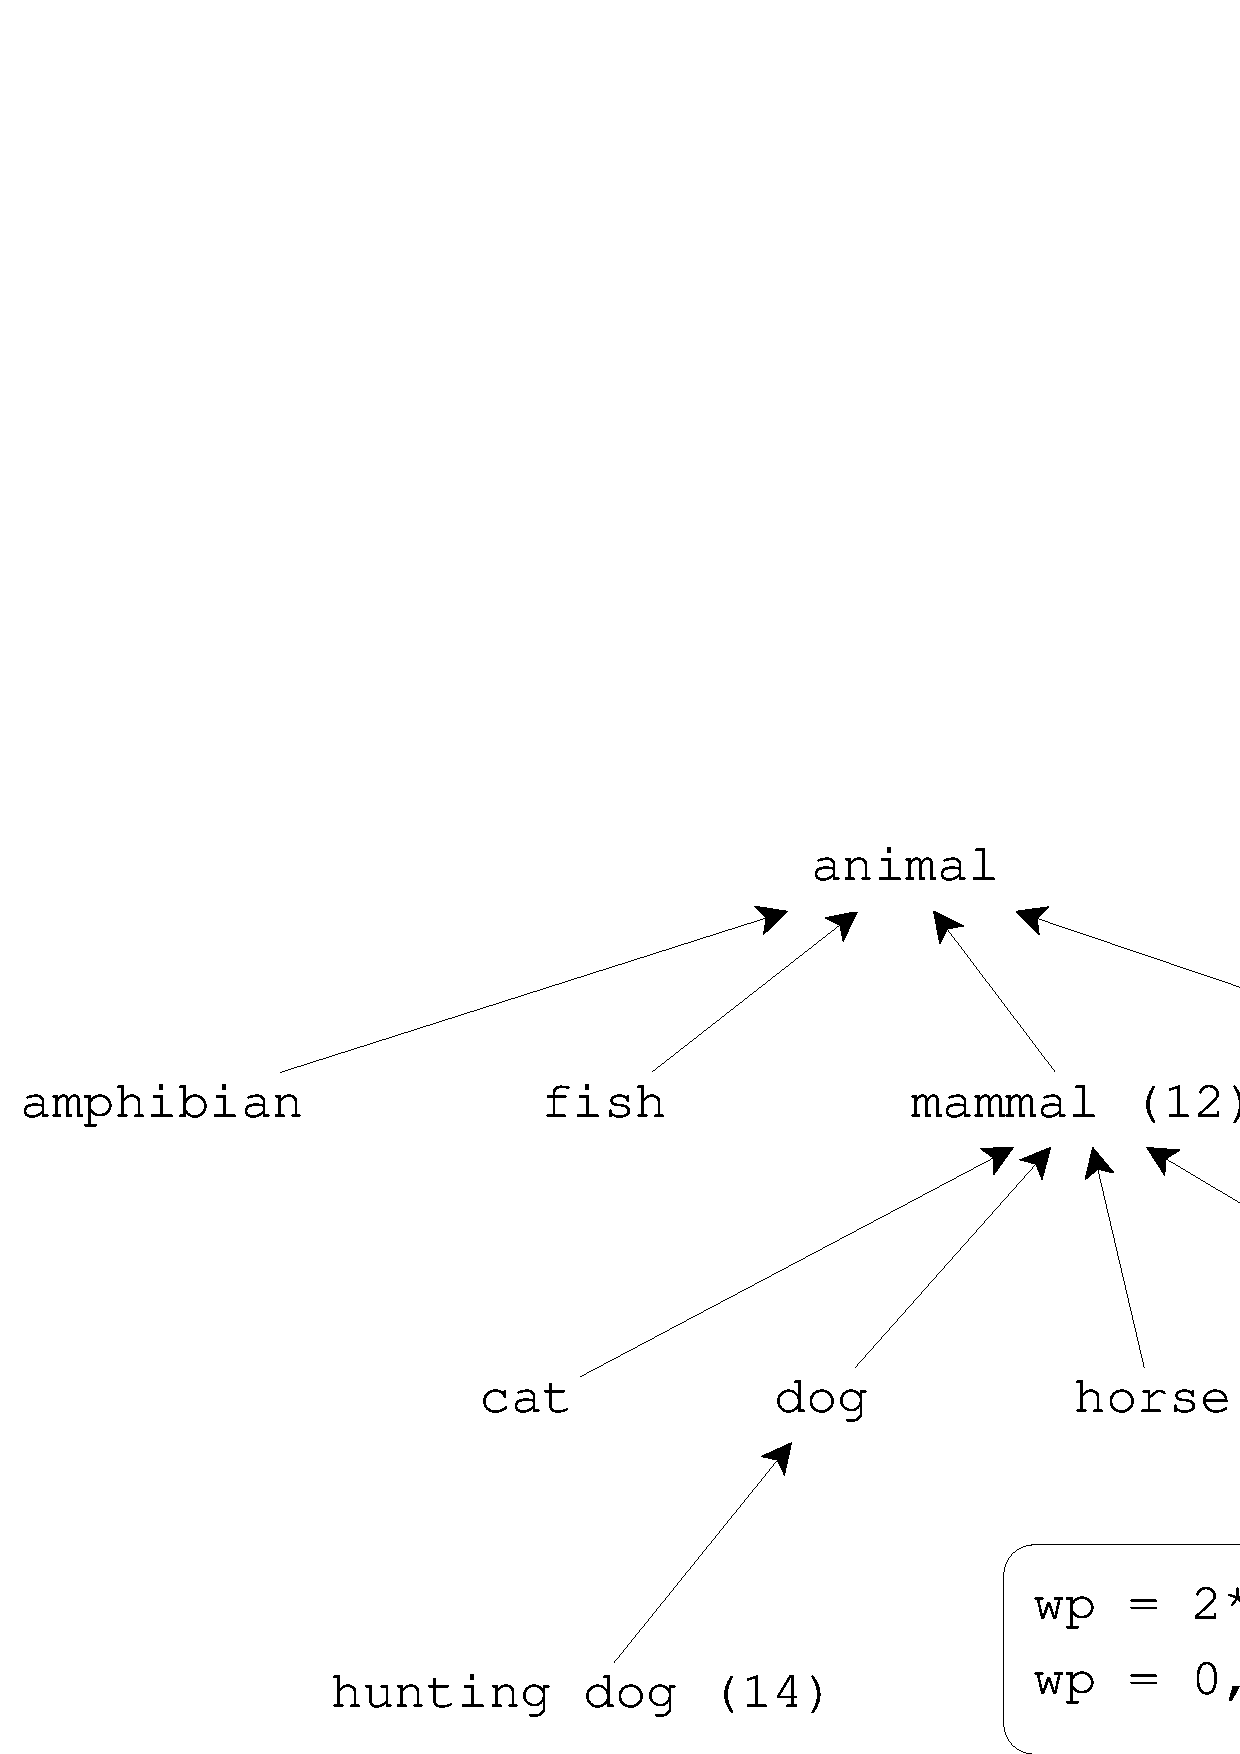
\includegraphics[width=0.65\textwidth]{fig-002.png}
 \caption{Gráfico com o número de estrofes por anagramático.}
 \label{fig02}
 \source{elaborada pelo autor.}
\end{figure}

Curiosamente, com essa relação entre o número de estrofes e palavras, é possível percebermos uma particularidade formal dos escritos de Romaguari, já que seus poemas são construídos por um grande número de estrofes, mas de tamanhos reduzidos, fazendo jus ao número de palavras desse autor-anagrama. Essa característica pode ser facilmente observada no poema “Cândida”, transcrito abaixo de \textcite[p. 235]{rosa_ave_1985}, composto por estrofes de dois versos e um esquema métrico de sete sílabas poéticas:

\begin{quote}
CÂNDIDA\\
(Marjolininha)

Candinha sonha comigo\\
no sonho sou seu amigo.

Eu que nunca vi Candinha\\
Reconheço-a na poesia.

Sonho que Candinha dorme\\
sonho que Candinha sonha

neste mundo certo e enorme\\
nesta vida não tristonha.

Candinha sonha um abrigo\\
no futuro - no conforme.

Que da simples alegria\\
o seu sonho se componha.

Candinha? Um sonho se sonha.
\end{quote}

Conforme vimos no gráfico da \Cref{fig01}, Sá Araújo Ségrim é o autor com o maior número de palavras, além de também apresentar um modelo formal característico, com menos divisão estrófica (\Cref{fig02}). Um exemplo representativo da estética de Ségrim pode ser o poema “Distância” \cite[p. 112]{rosa_ave_1985}, já explorado numa análise de \textcite{rossi_as_2007}, e com duas de suas estrofes transcritas a seguir. Como podemos ver, há uma diferença clara entre o estilo de Romaguari e o de Ségrim, denotada não apenas nos assuntos de que tratam os poetas, mas, sobretudo, na relação entre o número de palavras e o número de estrofes, detendo, este último, estrofes densas e sem esquema métrico definido, e, aquele, estrofes menores em número de palavras e estrato fônico marcado, nos termos de \textcite{ramos_fenomenologia_2011}. Soares Guiamar e Meuriss Aragão, por outro lado, mantém a quantidade de estrofes proporcional à quantidade de palavras escritas. Quanto ao primeiro, análises como a de \textcite{vital_uma_2021} e a de \textcite{rossi_as_2007} denotam que sua poesia, mesmo que não seja metricamente articulada, esconde importantes referências metapoéticas e exploração do estrato óptico do poema, isto é, a maneira como as palavras se distribuem na página. 

\begin{quote}
DISTÂNCIA

Um cavaleiro e um cachorro\\
viajam para a paisagem.\\
Conseguiram que esse morro\\
não lhes barrasse a passagem.\\
Conseguiram um riacho\\
com seus goles, com sua margem.\\
Conseguiram boa sede.\\
Constataram:\\
cai a tarde.

Sobre a tarde, cai a noite,\\
sobre a noite a madrugada.\\
Imagino o cavaleiro\\
esta orvalhada e estrelada.\\
O pensar do cavaleiro\\
talvez o amar, ou nem nada.\\
Imagino o cachorrinho\\
imaginário na estrada.\\
Caía a tarde.
\end{quote}

Como recurso a ser utilizado em análises qualitativas dos assuntos recorrentes nos poemas dos anagramáticos, propusemos a criação de nuvens de palavras (\textit{wordclouds}), gráficos que possuem o objetivo de representar visualmente, com o auxílio de diferentes tamanhos de fontes e cores, a frequência de palavras em determinado conjunto de textos \cite{jafar_framework_2012}. Para cada um dos autores, foi criada uma nuvem de palavras, procurando sintetizar os temas recorrentes em seus estilos poéticos (\Cref{fig03}, \Cref{fig04}, \Cref{fig05}, \Cref{fig06}). No \Cref{anexo}, há a lista das 10 palavras mais frequentes para cada anagramático.

\begin{figure}[h!]
 \centering
 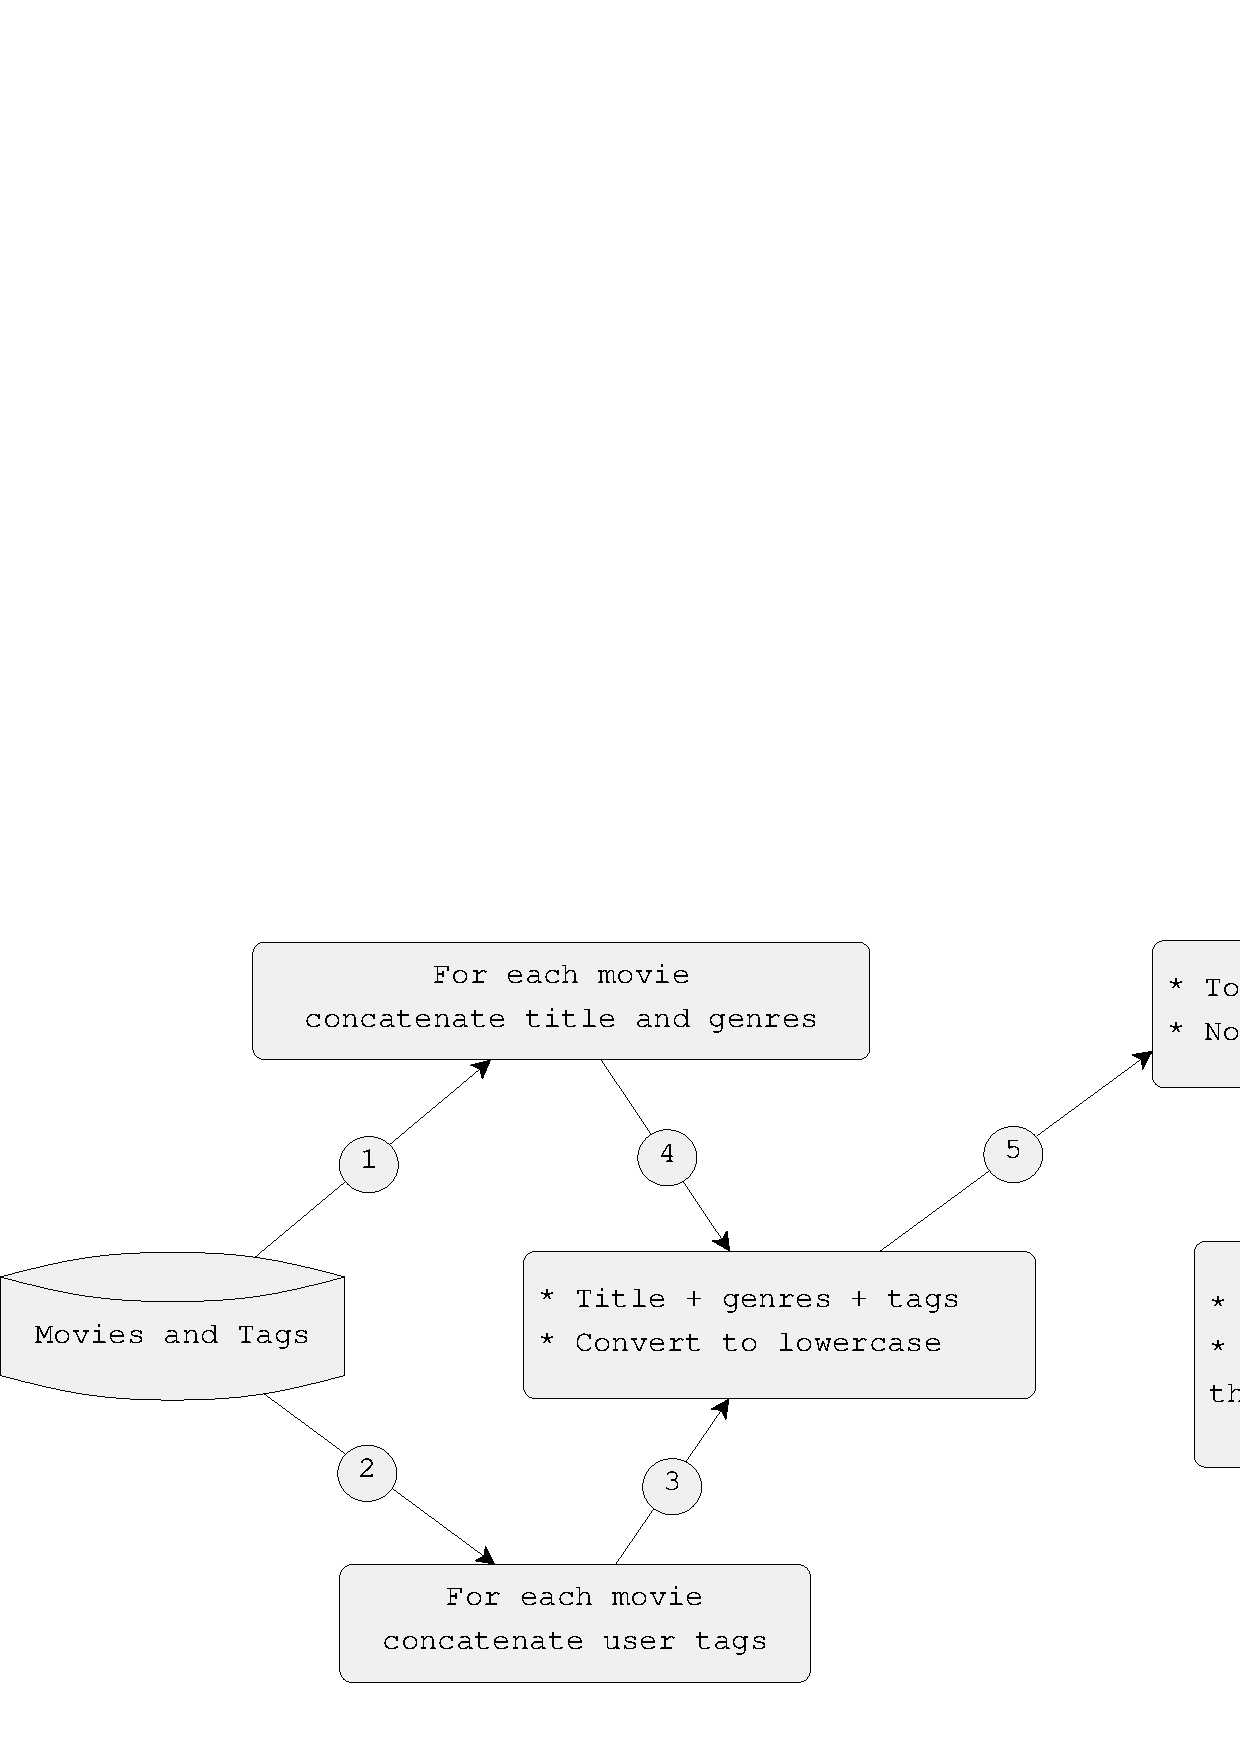
\includegraphics[width=0.85\textwidth]{fig-003.png}
 \caption{Nuvem de palavras dos poemas de Soares Guiamar.}
 \label{fig03}
 \source{elaborada pelo autor.}
\end{figure}

\begin{figure}[h!]
 \centering
 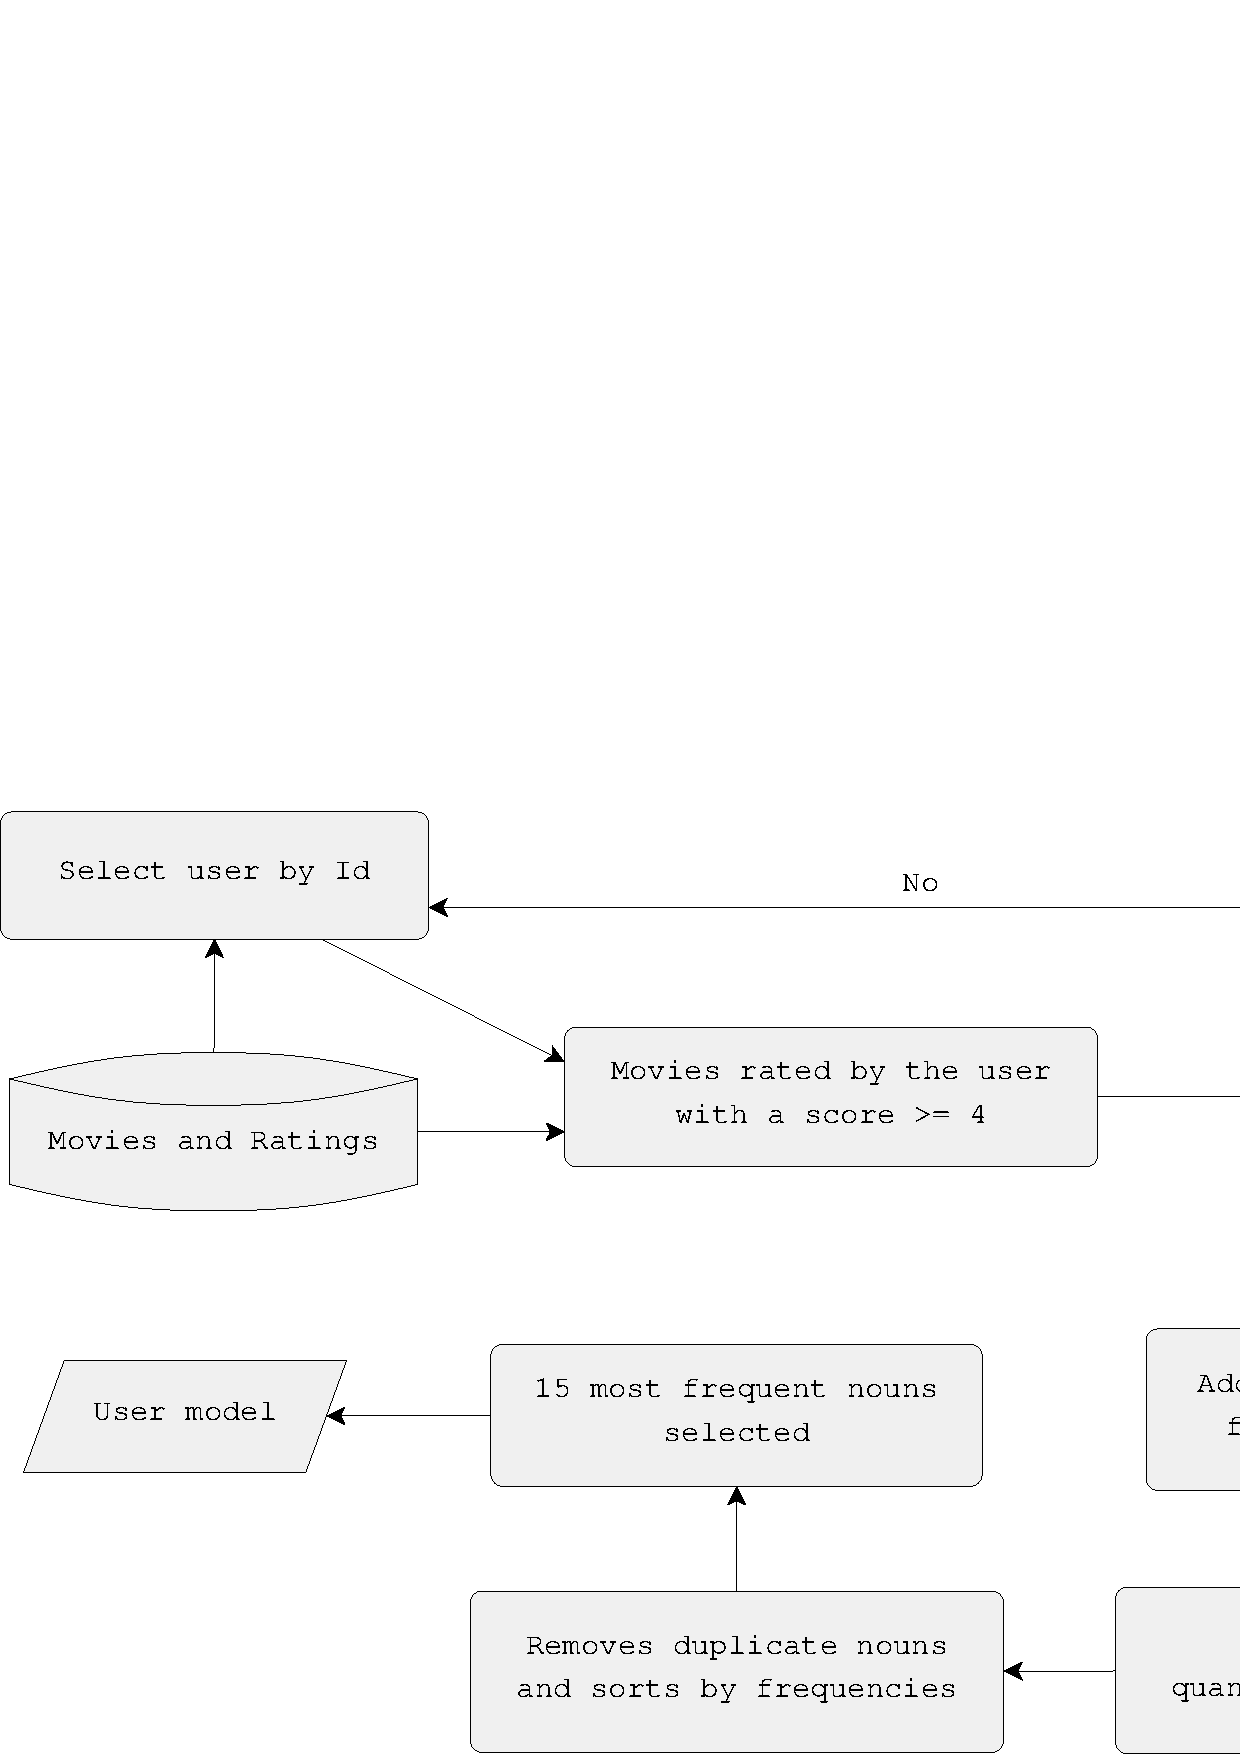
\includegraphics[width=0.85\textwidth]{fig-004.png}
 \caption{Nuvem de palavras dos poemas de Meuriss Aragão.}
 \label{fig04}
 \source{elaborada pelo autor.}
\end{figure}

\begin{figure}[h!]
 \centering
 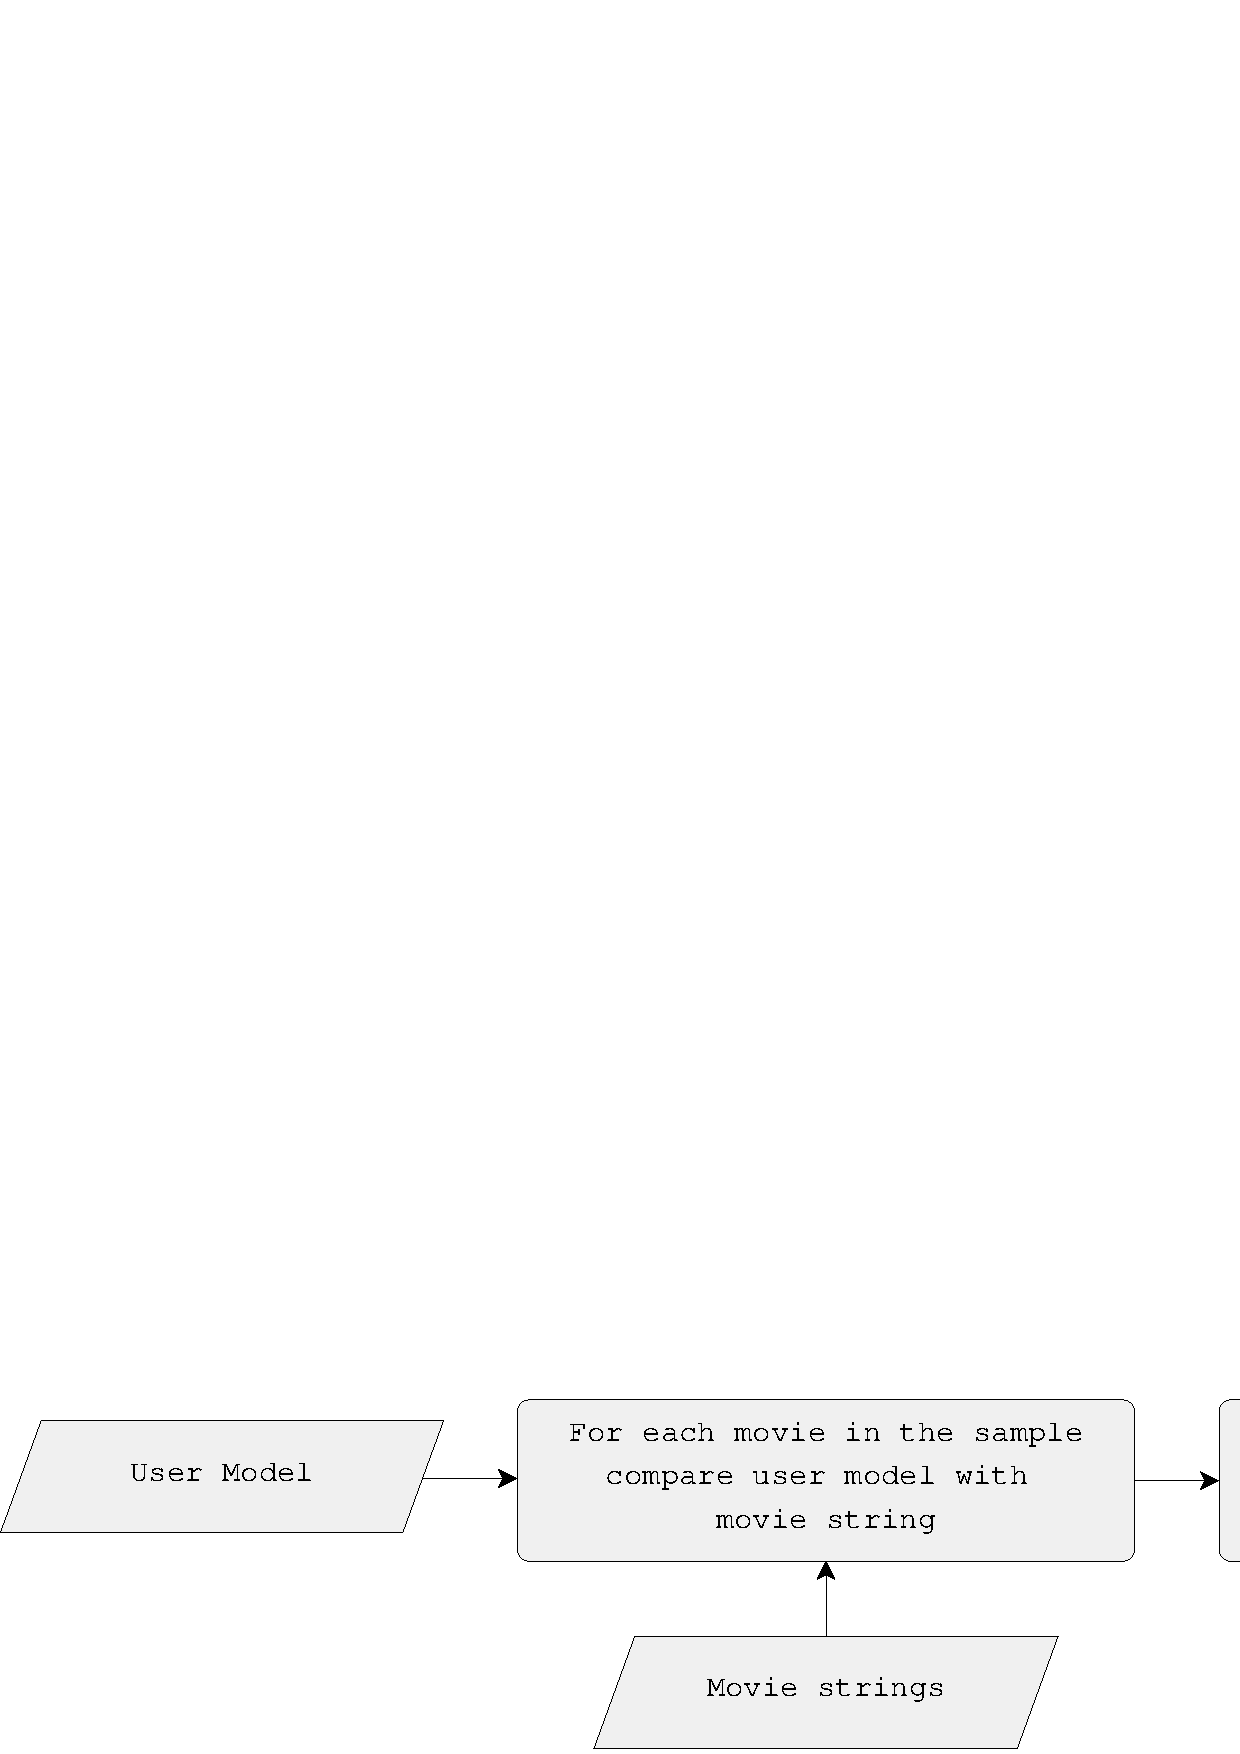
\includegraphics[width=0.85\textwidth]{fig-005.png}
 \caption{Nuvem de palavras dos poemas de Sá Araújo Ségrim.}
 \label{fig05}
 \source{elaborada pelo autor.}
\end{figure}

\begin{figure}[h!]
 \centering
 \includegraphics[width=0.85\textwidth]{fig-006.png}
 \caption{Nuvem de palavras dos poemas de Romaguari Sães.}
 \label{fig06}
 \source{elaborada pelo autor.}
\end{figure}

Após o processamento de todos os arquivos, chegamos às seguintes palavras mais frequentes nas obras: “onde”, “vida”, “mim”, “sempre”, “tarde”, “rio”, “mar”, “triste”. Neste ponto, salientamos que, sem os recursos computacionais da Linguística de \textit{Corpus} e suas interfaces com os Estudos Literários, tais resultados se tornariam exponencialmente trabalhosos, uma vez que a análise das palavras se dá \textit{token} a \textit{token}, isto é, uma a uma, e é realizada automaticamente pelo algoritmo criado. Na seção seguinte, são apontados breves caminhos de análise que conciliam a frequência das palavras com as epígrafes de cada autor-anagrama. 

\section{Discussão linguístico-literária}\label{sec-fmt-manuscrito}
Como dissemos acima, cada anagramático, em \textit{Ave, Palavra}, é introduzido por uma epígrafe que, em muitos casos, dialoga com o leitor a respeito do autor e dos poemas que se encontrarão nas próximas páginas. Essa pequena introdução se repete a cada momento em que Rosa nos apresenta a novos autores-anagrama. Em \textcite{brito_aspectos_2012}, há a informação de que os poemas da obra de 1970 foram publicados, originalmente, em edições do jornal O Globo, em 1961, o que, ao nosso ver, nos proporciona uma explicação a respeito da natureza das epígrafes, uma vez que o autor empírico, como que apresentando suas máscaras anagramáticas aos leitores d’O Globo, adiciona breves parágrafos sobre informações de seus “poetas de bolso”. A título de exemplo, a epígrafe de apresentação de Soares Guiamar, o primeiro dos anagramáticos, está transcrita, na íntegra, a seguir, e, num gesto ligeiro, acaba também por apresentar a ideia dos anagramas: “De Soares Guiamar – despercebido, impresso, inédito, fora de moda – que queria livro, o “Anagramas”, e disse palpites: Ser poeta é já estar em experimentada sorte de velhice. Toda poesia é também uma espécie de pedido de perdão” \cite[p. 58]{rosa_ave_1985}. 

Como vimos, os poemas de Guiamar representam boa parte da obra anagramática de Guimarães Rosa, uma vez que ele é o segundo poeta com o maior número de palavras e o primeiro no número de estrofes. Na sequência da obra, temos Meuriss Aragão, que é introduzido por uma epígrafe curiosa, pois é nela que Rosa relembra Soares Guiamar, restando poucas palavras para caracterizar Aragão: 

\begin{quote}
    Perguntam-me por mais versos de Soares Guiamar. Não são possíveis. Ele agora para \textbf{longe}, certo à beira do \textbf{Riachinho Sirimim}, \textbf{lugar} de se querer \textbf{bem}. Tenho, porém, outro poeta de bolso: Meuriss Aragão. Jovem, sem jeito, em sua primeira fase, provavelmente extinta. Vejam, se serve. \cite[p. 90, grifos nossos]{rosa_ave_1985}.
\end{quote}

Nessa apresentação, por sua vez, nos chamou a atenção a existência de palavras que se aproximam ou, em alguns casos, fazem parte daquelas mais frequentes na estética do primeiro autor-anagrama. Exemplos como “bem”, “lugar”, “Riachinho Sirimim” e “longe” dialogam diretamente com os termos mais frequentes resultados do processamento de seus poemas, que conta com termos como “bem”, “onde”, “mar” e “rio” como sendo bons representantes das 10 palavras mais frequentes (ver \Cref{fig03}). Ao mesmo tempo, Guimarães reserva pouco espaço para a entrada do próximo anagramático, Meuriss Aragão, que, inclusive, possui o menor número de palavras e estrofes de todos os quatro.

Neste ponto, caso não desejemos enquadrar as explicações anteriores apenas no terreno das coincidências literárias, é absolutamente relevante considerarmos as epígrafes e os trechos paratextuais como, juntamente dos poemas, veiculadores do sentido das obras. Revelar estes interstícios da forma literária, neste caso, só foi possível com a contagem de palavras e estrofes, e, desse modo, com os resultados do PLN. 

Da mesma forma, Rosa nos apresenta o terceiro dos autores-anagrama: Sá Araújo Ségrim, com a seguinte epígrafe:

\begin{quote}
    Poeta comprido – é outro dos anagramáticos, de que hoje disponho. Se bem talvez um tanto discípulo de Soares Guiamar, sob leves aspectos, sofre só e sozinho verseja. Sei que pensa em breve publicar livro: o ‘Segredeiro’, e do supracitado é, às vezes, o que prefiro. Será que conosco concordam? \cite[p. 112]{rosa_ave_1985}.
\end{quote}

Em primeiro lugar, nos chama a atenção o adjetivo “comprido”, utilizado para qualificar o poeta em questão. Tal qualidade é respaldada, por vezes, pelos resultados de nosso processamento, já que os poemas de Ségrim representam o maior número de palavras, sendo, dos quatro, o poeta mais comprido: 583 das palavras totais, isto é, 36,5\% do \textit{corpus}. Nessa mesma linha, a epígrafe salienta que Sá Araújo Ségrim é discípulo de Guiamar, outro dos anagramáticos, o qual possui o segundo maior número de palavras escritas: 527. Esta relação mestre-discípulo, além de se mostrar através da similaridade estrutural entre os dois autores – como é possível percebermos no número de palavras – há, na poesia de ambos, alta frequência dos termos “vida” e “rio”, que estão entre as 10 palavras mais frequentes para os dois anagramáticos. 

Num segundo momento, há a apresentação do segundo conjunto de poemas atribuídos a Ségrim. Na abertura, \textcite{rosa_ave_1985} faz as seguintes explicações a respeito da volta do anagramático, que, como sabemos, é seu preferido:

\begin{quote}
    Se lhe não firo a modéstia, direi, aqui, depressa, que Sá Araújo Ségrim, em geral, agradou. Por isso mesmo, volta, hoje, com novos poemas, que só não sei se escolhemos bem. Sendo coisas mui sentidas. Sendo o que ele não sabe da vida. Digam-me, o mais, amanhã. Leiam-no, porém \cite[p. 184]{rosa_ave_1985}.
\end{quote}

Segundo \textcite{rossi_as_2007}, os poemas de Ségrim comportam uma grande variedade tanto no nível formal quanto semântico. Nesse sentido, a divisão de suas poesias em dois agrupamentos situados em partes diferentes do livro fortalece a ideia da diversidade.

O último anagramático é Romaguari Sães, que foi publicado apenas em \textit{Ave, Palavra}, não tendo feito parte das publicações em jornal, como foi o caso dos outros autores-anagrama. De acordo com \textcite{rossi_as_2007}, Sães é o autor que mais se diferencia dos outros, impondo um estilo único e que se coloca em contato com trovas e cantigas medievais. Reforçando este ponto, a autora acrescenta que a escolha de palavras que se aproximam do campo semântico dessas produções, como “amigo”, “prado” e “bailai”, sugerem ainda mais a relação com a cultura medieval. Em sua epígrafe, lemos os seguintes trechos:

\begin{quote}
    Outro anagramático é Romaguari Sães, o ‘embevecido’, escondedor de poemas. No grupo, é considerado como um tanto diferente. Tem outra música. Tem um amor mais leve, originário, avançado. Disse, uma vez, em entrevista, que a poesia devia ser um meio de ‘restituir o mundo ao seu estado de fluidez, anterior, exempta’. Aprovam-no? \cite[p. 184]{rosa_ave_1985}.
\end{quote}

Como já apresentamos na seção de resultados, Romaguari conta com uma construção estrófica única em relação aos seus pares, produzindo um grande número de estrofes pequenas, em geral, metrificadas. Dentre as 10 palavras mais frequentes, citamos “prado”, também indicada por \textcite{rossi_as_2007} como um termo que aproxima sua estética da poesia medieval. 

Com isso, complementando os trabalhos a respeito das infindáveis obras de Guimarães Rosa, temos um panorama inicial da cooperação que alinha a Linguística de \textit{Corpus}, o PLN e o campo dos Estudos Literários, de modo a corroborar hipóteses interpretativas e lançar luz a recursos ainda pouco explorados na análise de obras literárias. Não obstante, a comparação realizada entre as máscaras anagramáticas de Guimarães Rosa se materializou através de tabela, gráficos e nuvem de palavras, recursos que poderão ser utilizados para estudos futuros do \textit{corpus} poético de \textit{Ave, Palavra}. Na tentativa de apontar os rumos interdisciplinares do contato inteligente entre as Ciências Exatas e as Humanidades, o presente estudo serve de base teórico-metodológica para o tratamento de textos literários, inclusive, em sala de aula, despontando interesses a partir de diversas disciplinas, como a Língua Portuguesa, a Literatura, a Programação e os conhecimentos lógicos. Nesse sentido, como denotado por \textcite{finatto_processamento_2015}, os conhecimentos empregados na compilação, anotação e processamento de dados de corpora podem ser complementados por estas áreas, além da associação acertada entre Linguística de \textit{Corpus} e PLN.
	
Em relação aos poemas processados, é de se considerar, ainda mais, o rigor (meta)poético empregado, a complexidade das características associadas a cada autor-anagrama e seus correspondentes formais, tanto na elaboração dos poemas quanto na criação das epígrafes. Tais fatos caminham na direção já discutida por \textcite{rossi_as_2007,vital_uma_2021}, que reconhecem a criação de máscaras anagramáticas na literatura rosiana como um objeto rico – embora pouco discutido pela crítica – mas que merece ser estudado em profundidade.

\printbibliography\label{sec-bib}
% if the text is not in Portuguese, it might be necessary to use the code below instead to print the correct ABNT abbreviations [s.n.], [s.l.]
%\begin{portuguese}
%\printbibliography[title={Bibliography}]
%\end{portuguese}


\appendix 

\section{Apêndice}\label{anexo}
\begin{table}[htbp]
\begin{threeparttable}
\caption{Ranking de palavras significativas mais frequentes para cada autor-anagrama.}
\label{tab02}
\centering
\begin{tabular}{p{2cm} p{2cm} p{2cm} p{2cm} p{2cm} p{2cm}}
\toprule
Ranking & Soares Guiamar & Meuriss Aragão & Sá Araújo Ségrim & Romaguari Sães & Corpus \\
\midrule
1 & bem & mim & tarde & candinha & onde \\
2 & vida & olhos & cavaleiro & maria & vida \\
3 & três & ti & noite & quero & mim \\
4 & moça & sempre & cachorro & sonho & sempre \\
5 & moço & som & conseguiram & meninas & tarde \\
6 & rio & céu & vida & sonha & rio \\
7 & então & onde & sol & prado & mar \\
8 & mar & saudade & rio & majolininha & triste \\
9 & onde & alma & distância & quanto & quero \\
10 & triste & fim & morro & vou & candinha \\
\bottomrule
\end{tabular}
\source{Elaborada pelo autor.}
\end{threeparttable}
\end{table}


\end{document}

